\documentclass{article}
\usepackage[german]{babel}
\usepackage{float}
\usepackage{fourier}
\usepackage[utf8]{inputenc}
\usepackage[T1]{fontenc}
\usepackage{amsfonts,amsthm, amsmath}
\usepackage{listings}
% The following is needed in order to make the code compatible
% with both latex/dvips and pdflatex.
\ifx\pdftexversion\undefined
\usepackage[dvips]{graphicx}
\else
\usepackage[pdftex]{graphicx}
\DeclareGraphicsRule{*}{mps}{*}{}
\fi

\setlength\parindent{0pt}
\lstset{language=Java}

\begin{document}

\textbf{Team:} TEAM 01, Falco Winkler (FW), Daniel Schruhl (DS)\\
\\
\textbf{Aufgabenteilung:}
\begin{itemize}
    \item
\end{itemize}

\textbf{Quellenangaben:}
\begin{itemize}
    \item Aufgabe 4, 11.06.2017, C. Klauck \& H. Schulz: \newline
    http://users.informatik.haw-hamburg.de/~schulz/pub/Verteilte-Systeme/AI5-VSP/Aufgabe4/
\end{itemize}

\textbf{Bearbeitungszeitraum:}
\begin{itemize}
	\item
\end{itemize}

\textbf{Aktueller Stand:}
\begin{itemize}
	\item
\end{itemize}

\textbf{Änderung des Entwurfs:}
\begin{itemize}
    \item Keine Änderungen
\end{itemize}

\newpage

\section{Einführung und Ziele}

\subsection{Randbedingungen}

\subsection{Kontextbegrenzung}

\newpage

\section{Gesamtsystem}

\subsection{Bausteinsicht}
%\begin{figure}[H]
%    \centering
%    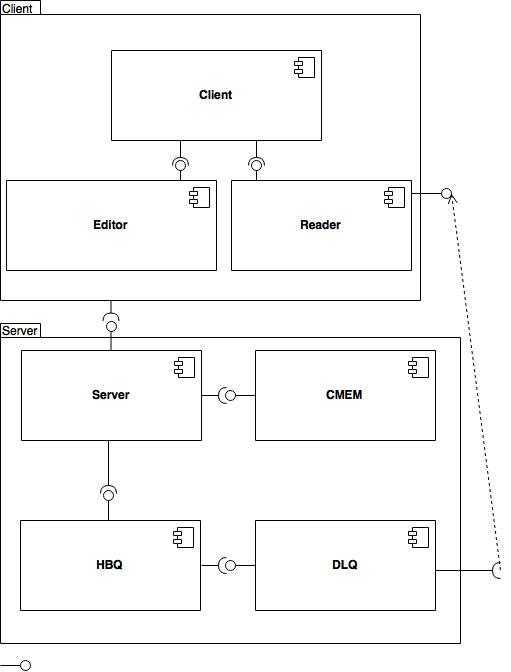
\includegraphics[width=0.5\textwidth]{component-diagram.png}
%    \caption[seq-dia]{Komponentendiagramm der ggT-App}
%    \label{fig:component-diagram}
%\end{figure}

\subsection{Laufzeitsicht}
%\begin{figure}[H]
%    \centering
%    \includegraphics[width=1.0\textwidth]{sequence-diagram.png}
%    \caption[seq-dia]{Eine ggT Berechnung mit Abbruch per Voting}
%    \label{fig:seq-diagram}
%\end{figure}

\newpage

\section{Subsysteme und Komponenten}

\end{document}